\chapter{计算机病毒的实验}

为了证明病毒攻击的可行性和它作为一个威胁的程度,我们进行了几个实验。在每种情况下,实验在知识和系统管理员的同意下进行。在进行实验的过程中,缺陷被小心地避免。这些实验不是基于实现失误,而是只在安全策略上存在缺陷,这是至关重要的。

\section{第一个病毒}

1983年11月3日,第一个病毒作为实验的构想是在一个每周举办计算机的安全研讨会上展示的。这一概念被作者研讨会第一次提出,“病毒”这个名称是伦恩·艾德曼想到的。经过8小时在VAX 11/750系统上负载运行Unix的专家工作,第一个病毒完成并准备好了演示。在一周内,得到许可后进行实验,5次实验得到了进行。11月10日,该病毒得到了安全研讨会的重视。

最初的感染是植入“vd”,这是一个以图形方式显示Unix文件结构的程序,并且通过系统公告栏向用户介绍。因为vd是系统上的一个新程序,我们不知道它的性能特征和其他操作的细节。病毒植入在程序的开始,因此在执行任何其他处理之前它就可以表现。


为了让攻击在一定的范围之内,需要采取一些预防措施。攻击者所进行的感染都是手动执行的,并且没有受到破坏,只进行报告。痕迹是用于确保病毒不会在没有检测之前进行传播,访问控制被用于感染过程,并且用于攻击的所需的代码放在片段里面,每个加密和保护用于防止非法使用。


在每五个攻击中,所有系统的权利在一个小时内授予给攻击者。最短的时间是在5分钟,平均时间在30分钟以内。即使是那些知道攻击的也会发生感染。在每种情况下,文件会进行“消毒”以保证不会侵犯了用户的隐私。虽然预计这次攻击会成功,但是这么短的控制时间还是非常令人惊讶的。此外,该病毒有足够快的速度(2/1秒以内),感染程序的延迟已经被忽略了。


实验的结果宣布后,管理员决定不允许在他们的系统上进行近一步的计算机安全实验。这个禁令包括计划研究可以跟踪潜在的病毒和密码的痕迹,这个实验可能在很大程度上改善安全性问题。这个反应是明显典型的恐惧,不试图解决技术问题的不适当性,往往选择不适当的策略解决方案。


在Unix系统上实验被成功的进行之后,很明显同样的技术在许多其他系统中也适用。特别的,实验计划实施在Tops-20系统、虚拟机系统和一个VM / 370系统,以及包含一些系统的网络中。在与管理员谈判的过程中,可行性在开发和测试原型中得到演示。对于Tops-20系统的原型的攻击是由一位经验丰富的Tops-20用户在6小时内开发出来的,一个VM / 370的新手用户在一个有经验的程序员的帮助下可以在30小时内完成,以及一个VM的新手用户在没有协助的条件下在20小时内完成。这些程序演示的是找到感染的文件、感染它们并且在用户边界交叉的能力。


经过几个月的谈判和管理方面的变化,最终决定实验不能允许进行。设施中的安全性官员反对安全性实验,甚至不阅读任何的提议。特别有趣的是,这让系统程序员及安全人员可以观察和监督所有实验的各个方面的内容。此外,系统管理员都不愿意用日志磁带的净化版本来离线分析病毒的潜在威胁,也不愿意让他们的系统程序员额外添加痕迹到系统中来帮助检测病毒的攻击。虽然这些行为没有明显的威胁,并且他们只需要一点时间、金钱和精力,管理员也不愿意允许调查。看起来,他们的反应与Unix管理员的恐惧反应是一样的。


\section{基于Bell-Lapadula的系统}

1984年3月,谈判是由对基于1108年面世的Univac电脑的Bell-LaPadula系统的实验表现的研究开始的。同意实验主要在几个小时内完成,但是花了几个月的时间才定下来。1984年7月,安排了一个两周期的实验。这个实验的目的仅仅是为了证明Bell-LaPadula基础上实现的一个原型系统中病毒的可行性。

因为极其有限的开发时间(由一个从未使用电脑的用户在一个五年内为使用1108的程序员帮助下,完成26小时的电脑使用),许多问题在实现中被忽略了。特别的,性能和攻击的一般性完全被忽略了。因此,每个感染需要花费约20秒时间,即使他们可以很容易地在一秒内完成。虽然痕迹可以用很少的经历在很大程度上得到消除,但是病毒的痕迹仍然要留在系统中。一次只有一个文件被感染,而不是同时感染许多文件。这使得病毒在没有涉及大量用户或程序的条件下,可以得到清楚的演示。作为一个安全预防措施,所使用的系统是一个专用的模式,只有一个系统盘、一个终端、一个打印机,并且账户只用于实验。


经过18个小时的连接时间,1108病毒进行了首次感染。在26小时的使用后,病毒是演示给了大约10个人,其中包括管理员、程序员和安保人员。病毒演示了跨用户边界的能力,从一个给定的安全级别转移到更高的安全级别。应该再次强调的是,这个活动中没有系统漏洞,但是Bell-LaPadula模型允许这类活动的合法性。


这次攻击不是很难执行。病毒的代码包括5行汇编代码、大约200行的Fortran代码和大约50行的命令文件。据估计,一个主管系统程序员可以在这个系统中于2周内编写一个更好的病毒。此外,一旦病毒攻击的本质被了解了,开发一个特定的攻击并不难。每个程序员现在都确信他们可以在同样的时间内建立一个更好的病毒(这是可信的,因为攻击者之前没有1108经验)。

\section{检测}

1984年8月初,测量共享和分析病毒蔓延的权限被授予给了VAX Unix系统。在这个时期的数据是非常有限的,但是出现了一些趋势。系统之间的共享程度似乎有很大区别,并且这些偏差被知道之前,许多系统已经进行了检测。少量的用户似乎占据了绝大多数的共享,并且可以通过保护它们使得病毒大大降低。保护少数的“社会”个人也可以减缓生物疾病。在检测没有发生之前感染也会发生的条件下,检测是保守的,所以估计攻击时间非常的缓慢。


由于这些系统的检测,识别了一组“社会”用户。一些结果使得几个主要的系统管理员惊讶了。系统管理员的数量是相当高的,如果他们被感染,整个系统可能在一个小时之内崩溃。一些简单的程序变化使得这种攻击降低了几个数量级而不改变功能。


图\ref{fig10}展示了两个系统,包括三类用户(S表示系统,A表示系统管理员,U表示正常用户)。“\# \#”表示每个类别中用户的数量,“传播”表示病毒传播到的用户的平均数量,而“时间”表示一旦登录给传播它们的平均时间,近似到最近的分钟数。平均时间是误导,因为一旦感染已经达到Unix上的‘根’账户,所有访问是允许的。考虑到这导致大约一分钟的时间是如此之快,感染时间成为感染传播速度的限制因素。这与
先前的实验结果一样使用的是一个实际的病毒。


\begin{figure}[h!]
    \centering
    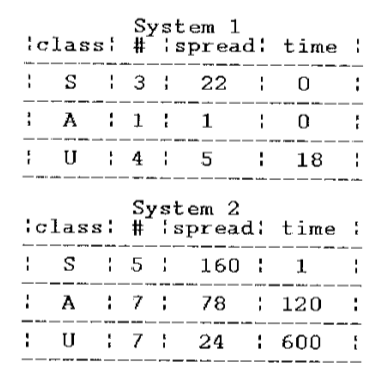
\includegraphics[width=0.40\textwidth]{figure/fig10.png}
    \caption{Summary of Spreading} 
    \label{fig10}
\end{figure} 

没有共享的用户在这些计算中忽略掉,但是其他的实验表明,任何用户都通过在系统上的公告板上提供程序来与其他用户进行共享。详细的分析表明,系统管理员倾向于尝试那些刚刚发布的程序。这允许普通用户在几分钟内感染系统文件。管理员帐户用于运行其他用户的程序和存储一般系统的可执行文件和一些普通用户拥有的非常常用的文件。这些条件使得病毒攻击可以很快进行。系统管理员的独立账户的使用,正常使用和系统的常用程序运动(验证之后)到系统区域也被考虑在内。

\section{总结与结论}

图\ref{fig11}总结了上述以及其他实验的结果。系统在水平轴上(Unix、Bell-LaPadula),而纵轴显示性能(编程时间、感染时间、代码行数、实验执行次数、最低占据时间、平均占据时间和最大占据时间),占据时间表明,在将延迟引入病毒之后,攻击者攻击者的所有特权将得到保障。

\begin{figure}[h!]
    \centering
    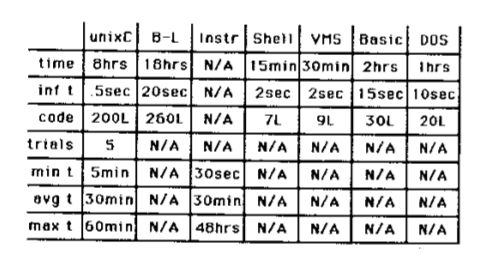
\includegraphics[width=0.60\textwidth]{figure/fig11.png}
    \caption{Experimental Results} 
    \label{fig11}
\end{figure} 

病毒攻击在很短的时间内似乎很容易发展,也可以设计成在最新的系统中几乎没有痕迹,在现代多级安全策略使用中是有效的,并且只需要最少的专业知识来实现。它们的潜在的威胁是严重的,它们可以通过电脑系统进行很快的传播。这样看来,他们可以用在电脑之间传播的方式,在电脑网络之间传播,这样对当前的许多系统形成了一个广泛而相当直接的威胁。


防止控制安全实验的问题是明确的;拒绝用户继续他们的工作促进非法攻击;并且如果一个用户在没有使用系统漏洞和专门知识的前提下就可以发动以此攻击,这说明其他用户也可以。简单地告诉用户不要发动攻击,只能有很小的效果。可以信任的用户不会发动攻击,而造成破坏的用户不能信任,所以只有合法工作受到阻碍。一个观点说,允许用于降低安全性的攻击在作者看来是一个谬论。利用攻击来学习的想法甚至只能在政府政策允许的安全的系
统上进行\upcite{16,17}。更加理性的是,使用开放和
控制实验作为资源来提高安全性。


